
\section{Background}
\label{sec:bg}

Task scheduling introduces several fundamental concepts.

\subsection{Periodic task and schedule}
~

Firstly, a periodic task $\tau_i(C_i, D_i, T_i)$ is characterized 
by its worst-case execution time (wcet) $C_i$, its deadline $D_i$, and 
its period $T_i$. This definition can be expanded by including an 
initial offset, which corresponds to the time of the task's first 
execution, and an activation offset, which is the time delay between 
the task being ready to execute (i.e., its execution period has begun) 
and the task actually starting to run. Secondly, a schedule $S$ is a 
function that assigns a boolean value for each task $\tau$ and each 
time tick $t$, indicating whether the task $\tau$ is running at 
time $t$. Therefore, a scheduling algorithm is the method that, 
given a set of tasks, produces a schedule $S$ for the task set.

This task model and schedule definition are widely adopted in the literature (see section \ref{sec:literature}) 
and are the building blocks of all scheduling algorithms.
The periodic task model, in particular, is used to define more complex
tasks such as DAG tasks (see below) that will be used as input in the 
machine learning model (see section \ref{sec:methodology}).

\subsection{DAG task}
~

A Directed Acyclic Graph (DAG) task 
is a task that models the multiple subtasks of an chain of tasks
that have a precedence constraints.
For example, when considering the task $\tau_1$ that makes an 
aircraft keep its altitude, you usually have a number of subtasks
to handle this task, namely : reading from the altitude sensor ($\tau_{11}$),
reading for the speed sensor ($\tau_{12}$), computing the new speed for the aircraft
to keep its altitude ($\tau_13$), computing the amount of thrust needed to achieve
this new speed ($\tau_14$), and finally actuating the aircraft's jet engine ($\tau_15$).
In this example, the DAG for $\tau_1$ can be seen in Figure \ref{fig:dag_example}.

\begin{figure}
    \centering
    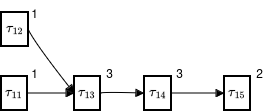
\includegraphics[width=0.5\linewidth]{images/example_dag.png}
    \caption{DAG task $\tau_1$. The nodes are the subtasks,
    the edges of the graph represent the precedence constraints between each subtasks and the worst-case execution time (wcet) of each subtask written as an exponent.}
    \label{fig:dag_example}
\end{figure}

A DAG task $\tau_i$ also has a period $T_i$ and a wcet $C_i$ which 
is the sum of its subtasks wcets, and a deadline $D_i$.
For instance, according to Figure \ref{fig:dag_example},
the wcet for $\tau_1$ is 10 time units.
You can also see how, for $\tau_1$, 
the subtasks $\tau_{12}$ and $\tau_{11}$ can be parrallelized (i.e., 
executed in parallel) but the subtask $\tau_{13}$ needs to wait 
for both $\tau_{11}$ and $\tau_{12}$ to finish their execution 
before it can start running.
\\

This concept will be the task model used in to conduct 
part of the systematic literature review (see Section \ref{sec:literature})
and it also will be the task model used for designing 
the machine learning model (see Section \ref{sec:methodology}).


\subsection{Utilization factor}

The utilization factor represents the percentage of processing 
time that a taskset $(\tau_1, \cdots, \tau_n)$ will utilize. 
Formally, it is defined as
\begin{align}
U = \sum_{k=1}^{n} \frac{C_k}{T_k}
\end{align}
where $U$ is the utilization factor. This concept is significant 
because, when evaluating a scheduling algorithm $S$, we desire 
$S$ to effectively schedule tasksets that maximize the utilization 
factor $U$. Consequently, the higher the utilization factor bound 
for $S$, the more efficient the scheduling algorithm. Additionally, 
this concept is valuable in real-time systems where processing 
resources are often limited and expensive, making it crucial to 
maximize their usage.

This concept is also used either as a measurement
when comparing two scheduling algorithms 
and considering their utilization bound(see Section \ref{sec:literature}),
or used as a parameter to generate tasksets or DAG tasks with 
a fixed utilization (see Section \ref{sec:methodology}).

\subsection{Makespan}

The makespan or end-to-end response time of a 
DAG task is the amount of time it takes for all the subtasks
in the DAG task to finish executing when given a schedule.
For instance, for the task $\tau_1$ shown in Figure \ref{fig:dag_example},
the makespan of $\tau_1$ for the schedule shown in Figure \ref{fig:schedule_example}
is 9.
Notice that in Figure \ref{fig:schedule_example},
if the subtasks $\tau_{11}$ and $\tau_{12}$ were executed 
sequentially instead of in parrallel, the makespan would be 
one time unit longer, in this case 10 instead of 9.

\begin{figure}
    \centering
    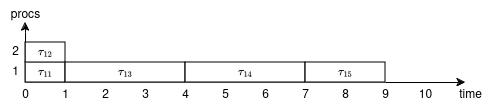
\includegraphics[width=0.5\linewidth]{images/schedule_example.png}
    \caption{Example of schedule for $\tau_1$. The y axis represents the number
    of processors that are not idle. For the first two subtasks there are two processors
    active and for the rest there is only one active processor.}
    \label{fig:schedule_example}
\end{figure}

This is a key measurement when dealing with DAG tasks (see Section \ref{sec:literature})
and it will be the main efficacy criteria when comparing 
the machine learning model with state-of-the-art heuristics and ILP
(see Section \ref{sec:methodology}).

\subsection{Capacity augmentation bound}

Another measurement used when scheduling event-chains, or DAG, tasks  
is the capacity bounds, or capacity augmentation bound,
which compares resource use to an theoretically optimal scheduling algorithm.
It can also be used as a simple schedulability test.
The matehmatical definition for a scheduling algorithm $S$ of its capacity
augmentation bound $\beta$ is that, for any chain of events represented by a DAG $G$
satisfying the following condition :
\begin{align}
    \beta \times U \leq m \wedge  \beta \times len(G) \leq D,
\end{align}
the associated DAG is schedulable by $S$.
Here, $len(G)$ is the length of the longest path, in terms of WCETs,
in the graph $G$, $D$ is the DAG task's deadline, $m$ the number of processors and $U$
is the utilization factor of the DAG task (with the WCET of the DAG being the sum of all tasks' WCET).
As you can see, the lower $\beta$ is, the better the scheduling algorithm.\\
This metric is used for DAG tasks or event-chains of tasks.

%\cite{tiryaki2006sunit} is really good with MAS but really bad with something else.
\subsection{Optimality}

A scheduling algorithm $S$ is said to be optimal 
when the following condition is true:
for every taskset $\Omega$, if there exists 
a scheduling algorithm $S'$ so that $\Omega$ is feasible by $S'$,
then $\Omega$ is also feasible by $S$.
Where {\it{feasible}}, 
means that, using the schedule generated by $S$,
all the tasks in the taskset will finish executing before their deadlines.

This concept is used in the literature, mainly for independent tasks scheduling
(see Section \ref{sec:literature}).

\subsection{Acceptance ratio}

When dealing with several independent DAG tasks
or tasksets, 
the acceptance ratio is often used to measure the 
performance of a scheduling algorithm (see Section \ref{sec:literature}).
It consists of looking at a number of generated tasksets (or DAG tasks)
and calculating the amount of schedulable (i.e., 
the schedule produced doesn't lead to a deadline miss) tasksets compared to 
the total amount of taskets.
The resulting percentage is the acceptance ratio 
and the closer it gets to 100\% for a scheduling algorithm, the better the scheduling algorithm.

This concept is also used as a metric, to assert the efficiency
of scheduling algorithms when considering independent tasks (see Section \ref{sec:literature}).
\\


While the acceptance ratio, also called system schedulability, is used 
to measure the performance of scheduling alrogithms for independent tasks,
the makespan and the capacity bound are only used for DAG tasks and tasksets representing chain of events.

\subsection{RM and EDF scheduling}
~

When designing a scheduling algorithm, the key decision involves 
determining which task should execute first when two or more 
independent tasks are ready to execute. This requires assigning each 
task a priority. \cite{liu1973scheduling} introduced two 
heuristics for this purpose: Rate Monotonic (RM) and Earliest 
Deadline First (EDF).

The RM algorithm is a fixed-priority scheduling algorithm, 
meaning that the priority of each task is known before execution 
begins. RM assigns the highest priority to tasks with the minimum 
execution rate, i.e., $\frac{C_k}{T_k}$, and is considered optimal 
for assigning fixed priorities to tasks. In contrast, EDF assigns 
priorities dynamically by selecting tasks based on which one has 
the earliest absolute deadline.

Figure \ref{fig:edf_rm_examples} illustrates the difference 
between the two algorithms by scheduling the same two tasks, 
$\tau_1$ and $\tau_2$. $\tau_1$ has a worst-case execution time of 0.5 time units 
and a period of 2 time units, while $\tau_2$ has a worst-case execution 
time of 2 time units and a period of 3 time units. These are 
examples of implicit deadline tasks, where the relative deadline 
equals the end of their execution period. 

\begin{figure}
    \centering
    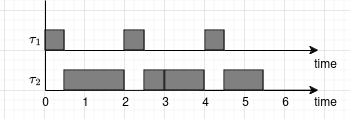
\includegraphics[width=\linewidth, height=100px]{images/schedule_rm.png}
    a)
    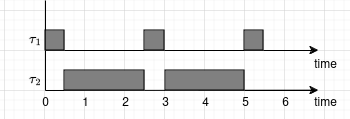
\includegraphics[width=\linewidth, height=100px]{images/schedule_edf.png}
    b)
    \caption{Schedules of $\tau_1$ and $\tau_2$ using Rate Monotonic (a)
    and Earliest Deadline First (b) heuristics.}
    \label{fig:edf_rm_examples}
\end{figure}

Although EDF calculates each priority at runtime, it is optimal 
for uniprocessor scheduling and has a theoretical utilization bound 
of 1, which is the maximum possible for a feasible taskset on a 
single processor. RM, on the other hand, has a much lower 
utilization bound than EDF. While one might argue that RM introduces 
less runtime overhead and is therefore more practical, it has been 
shown that RM leads to more task preemptions (interrupting the 
execution of a task, as seen at times 2 and 4 for task $\tau_2$ in 
Figure \ref{fig:edf_rm_examples}.a). This, combined with its lower 
utilization bound and non-optimality, makes EDF perform better than 
RM\cite{buttazzo2005RMvsEDF}.

Although \cite{liu1973scheduling}'s work focused on uniprocessor 
systems, the proposed algorithms have also been applied to 
multi-processor scheduling.
For example, Global EDF (GEDF)
can be used on multi-core systems when allowing task migrations
and Partitioned EDF (PEDF) is used when forbidding task migrations
(The RM equivalents also exist).